\chapter{Entity and mapping translation}
% what is all needed (+table comparison)
% abstraction and wrappers (generally)
% algorithm pseudocodes - builder+ parser for mappings, visitor for queries
% working with the abstract classes, not concrete implementation
% concrete example dapper -> something complex (NH/EF)
% all theory - no limit of implementation (DB querying is present etc)
% special cases

We will begin by examining entities and their database mapping. Although the frameworks analyzed earlier differ in syntax and configuration approaches, they nonetheless share several common patterns. The aim of this chapter is to identify these common concepts and to design a unified abstraction. This abstraction should be expressive enough to capture all mapping capabilities while remaining independent from any specific implementation. Once the abstraction is defined, we can focus on developing algorithms that support its translation.

\section{Defining abstraction}

Let us begin with the entity itself. At its core, it is a plain C\# class composed of properties. Typically, such a class corresponds to a single database table, with each property representing a directly loaded or transformed column value. The mapping must describe this relationship explicitly. In many cases, class and property names serve as defaults, but when they diverge from their database identifiers, aliases must be specified. The .NET type system does not fully align with that of database systems. While the property's type and nullability often provide sufficient hints, more specific constraints---such as length, precision or character encoding---require explicit configuration.

And of course, a table rarely exists in isolation. In a relational model, it is typically connected to others through defined relationships. The mapping must at least capture primary and foreign keys to allow proper navigation. More complex associations often require further configuration. An \acrshort{orm} may need to know which side owns the relationship, how cascading behaviour is handled, or how orphaned entities are treated.

It is worth noting that features operating purely on the database side such as indexes, triggers, or computed columns are generally outside the scope of entity mapping. Some \acrshort{orm}s allow limited representation of those features, but we will not consider them in the abstraction.

After our examination in \autoref{chapter:ormcomparison}, we built \autoref{tab:entity_mapping}. First, we identified important parts of entity mapping, each represented by a table row. Each column depicts a different \acrshort{orm} and how the specific mapping is implemented. We did not consider all possible mapping formats and proceeded with those selected in \autoref{sec:perf_eval}. 

From the table rows, it is evident that the most important mapping concepts include \textbf{table} and \textbf{schema names}, the names, types, and nullability of \textbf{columns}, as well as column \textbf{constraints} such as length, scale, and precision. Furthermore, \textbf{primary keys} with their respective strategies for generation and \textbf{foreign keys} along with their cardinalities emerged as significant factors for relationships.

%\clearpage
\begin{landscape}
\begin{table}
\centering
\caption{Configuration examples for key entity mapping aspects.}
\label{tab:entity_mapping}
\scriptsize
\def\arraystretch{1.35}
\begin{tabular}{
>{\raggedright\arraybackslash}p{20.00mm}
>{\arraybackslash}p{30.00mm}
>{\arraybackslash}p{30.00mm}
>{\arraybackslash}p{30.00mm}
>{\arraybackslash}p{30.00mm}
>{\arraybackslash}p{40.00mm}
>{\arraybackslash}p{30.00mm}
}
\toprule
  &    \textbf{Dapper}\newline no mapping &  \textbf{PetaPoco} \newline attribute mapping &    \textbf{RepoDB} \newline attribute mapping &   \textbf{LINQ to DB} \newline fluent mapping & \textbf{NHibernate} \newline XML file mapping  &   \textbf{EF Core} \newline attribute mapping \\
\midrule
Primary key  & - & \texttt{[PrimaryKey]} on class & \texttt{[Primary]} on property & HasPrimaryKey() & \texttt{<id name="OrderID" column="" type="">\ldots</id>} & \texttt{[Key]} on property \\

\midrule
Foreign key & – & – & – & \texttt{.Association()}  & in \texttt{one-to-many} & \texttt{[ForeignKey]} \\

\midrule
Table and schema &
– &
\texttt{[TableName("x.y")]} &
\texttt{[Table("y", Schema="x")]} &
\texttt{HasSchemaName("x")} \newline \texttt{HasTableName("y")} &
\texttt{<class table="y" schema="x">} &
\texttt{[Table("y", Schema="x")]} \\

\midrule
Database type & derived from property & derived from property & \texttt{[DbType]} & \texttt{.HasDbType()} & \texttt{type="decimal"} & \texttt{[Column(TypeName="")]} \\

\midrule
Precision & – & – & \texttt{[Precision]} & \texttt{.HasPrecision()} & \texttt{precision="18" scale="2"} & \texttt{[Precision(18,2)]} \\

\midrule
Nullability & derived from property & derived from property & \texttt{[IsNullable(true)]} & \texttt{.IsNullable()} & \texttt{not-null="false"} & derived from property \\

\midrule
One-to-one & – \newline (join + \texttt{splitOn}) & – \newline (join + \texttt{Fetch<T1,T2>}) & – \newline (\texttt{QueryMultiple}) & \texttt{.Association()} and mapped keys & \texttt{<bag> <key column=""/> <one-to-one class="" column=""/> </bag>} & mapped keys and derived from property type \\

\midrule
One-to-many & – \newline (join + \texttt{splitOn}) & – \newline (join + \texttt{Fetch<T1,T2>}) & – \newline (\texttt{QueryMultiple}) & \texttt{.Association()} and mapped keys & \texttt{<bag> <key column=""/> <one-to-many class="" column=""/> </bag>} & mapped keys and derived from property type \\

\midrule
Many-to-many & – \newline (join + \texttt{splitOn}) & – \newline (join + \texttt{Fetch<T1,T2>}) & – \newline (raw SQL + in memory) & \texttt{.Association()} and mapped keys  & \texttt{<bag> <key column=""/> <many-to-many class="" column=""/> </bag>} & fluent join-table definition:\newline\texttt{UsingEntity("", l => l.$\cdots$, r => r.$\cdots$)} \\
\bottomrule
\end{tabular}
\end{table}
\end{landscape}

\section{Intermediate representation}
%diagram fo design and specific parts
Building on the mapping aspects identified above, we now introduce a unified intermediate representation. This abstraction captures both application-level and database-level details of entity mapping in a structured and extensible manner. The complete conceptual model is illustrated in the \acrshort{uml} diagram in \autoref{fig:abstract_ir}.

\begin{figure}[H]
  \centering
  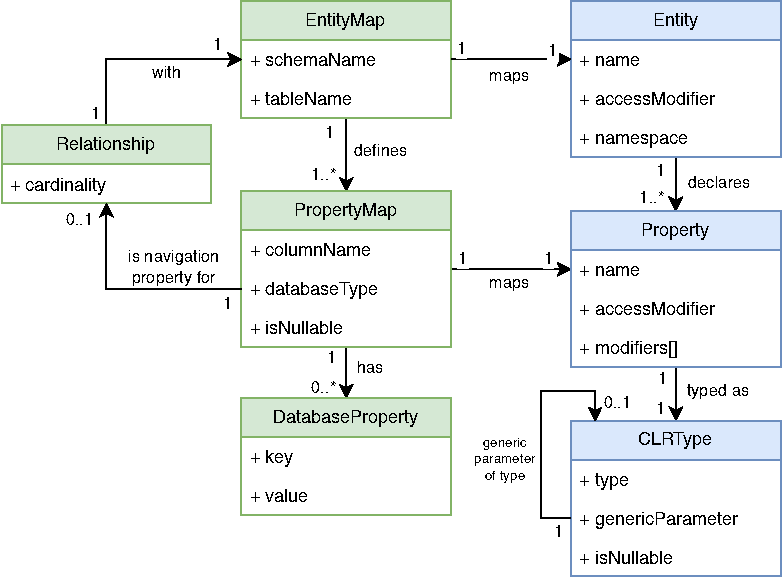
\includegraphics[scale=1]{thesis/img/thesis/04_abstract_ir.drawio.pdf}
  \caption{Class diagram of intermediate representation of entity mapping.}
  \label{fig:abstract_ir}
\end{figure}

The starting point for mapping is the representation of a C\# class itself, encapsulated in the \texttt{Entity} class. This class holds information about the entity's name, its access modifiers, and namespace. Additionally, the \texttt{Entity} references all individual properties it contains. Each property is represented using the \texttt{Property} class, which includes its access modifiers, data type, and name. 

Type information is extracted into the \texttt{CLRType} class (\acrshort{clr} referring to \acrlong{clr}) to allow nesting in a generic parameter. Such generics commonly appear in navigation properties for relationships, as .NET typically represents one-to-many or many-to-many relationships by collections (e.g. \texttt{List} or \texttt{HashMap}) parameterized by the target entity type. The classes \texttt{Entity}, \texttt{Property} and \texttt{CLRType} collectively represent the application-level aspects of the entity.

Additional classes must be introduced for database mapping purposes. At the core of data mapping representation is the \texttt{EntityMap} class, which acts as the primary container linking an entity class to a specific database table, namely schema and table names. Each entity property is mapped separately to its corresponding database column through the class \texttt{PropertyMap}, which stores details such as column name and its associated database data type.

When an entity property represents a foreign key, additional details about the cardinality and the target entity of the relationship must also be stored. These details are explicitly handled by the \texttt{Relationship} class. Additionally, the more complex features of column mapping---such as type constraints and other specialized attributes---are represented using the flexible \texttt{DatabaseProperty} class. This class maintains information in key-value pairs. For example, a decimal property type like \texttt{DECIMAL(15,8)} would be represented by  keys `Precision' and `Scale', holding values 15 and 8, respectively. And the base type `decimal' would go under \texttt{database type}. 

%The relationship between EntityMap and Entity has $1 \rightarrow 1$ multiplicity, but it could be modified to $1 \rightarrow *$ in the rare case of one entity mapping multiple tables.


\section{Abstract entity builder}

 \begin{lstlisting}[caption=AbstractEntityBuilder, language=pseudo]
abstract class AbstractEntityBuilder
    
public: 
    AddPrimaryKey(propertyName, strategy) {...}
    AddForeignKey(propertyName, cardinality, target) {...}
    AddTable(tableName) {...}
    AddSchema(schemanName) {...}
    AddNamespace(namespace) {...}
    AddClassHeader(modifier, className) {...}
    AddProperty(name, type, modifiers) {...}
    AddPropertyMapping(propertyName, databaseProperties) {...}
    
public:
    abstract Build();
private: 
    abstract BuildImports();
    abstract BuildTableSchema();
    abstract BuildPrimaryKey();
    abstract BuildForeignKey();
    abstract BuildProperties();
    abstract FinalizeBuild();
 \end{lstlisting}


\begin{figure}[H]
  \centering
  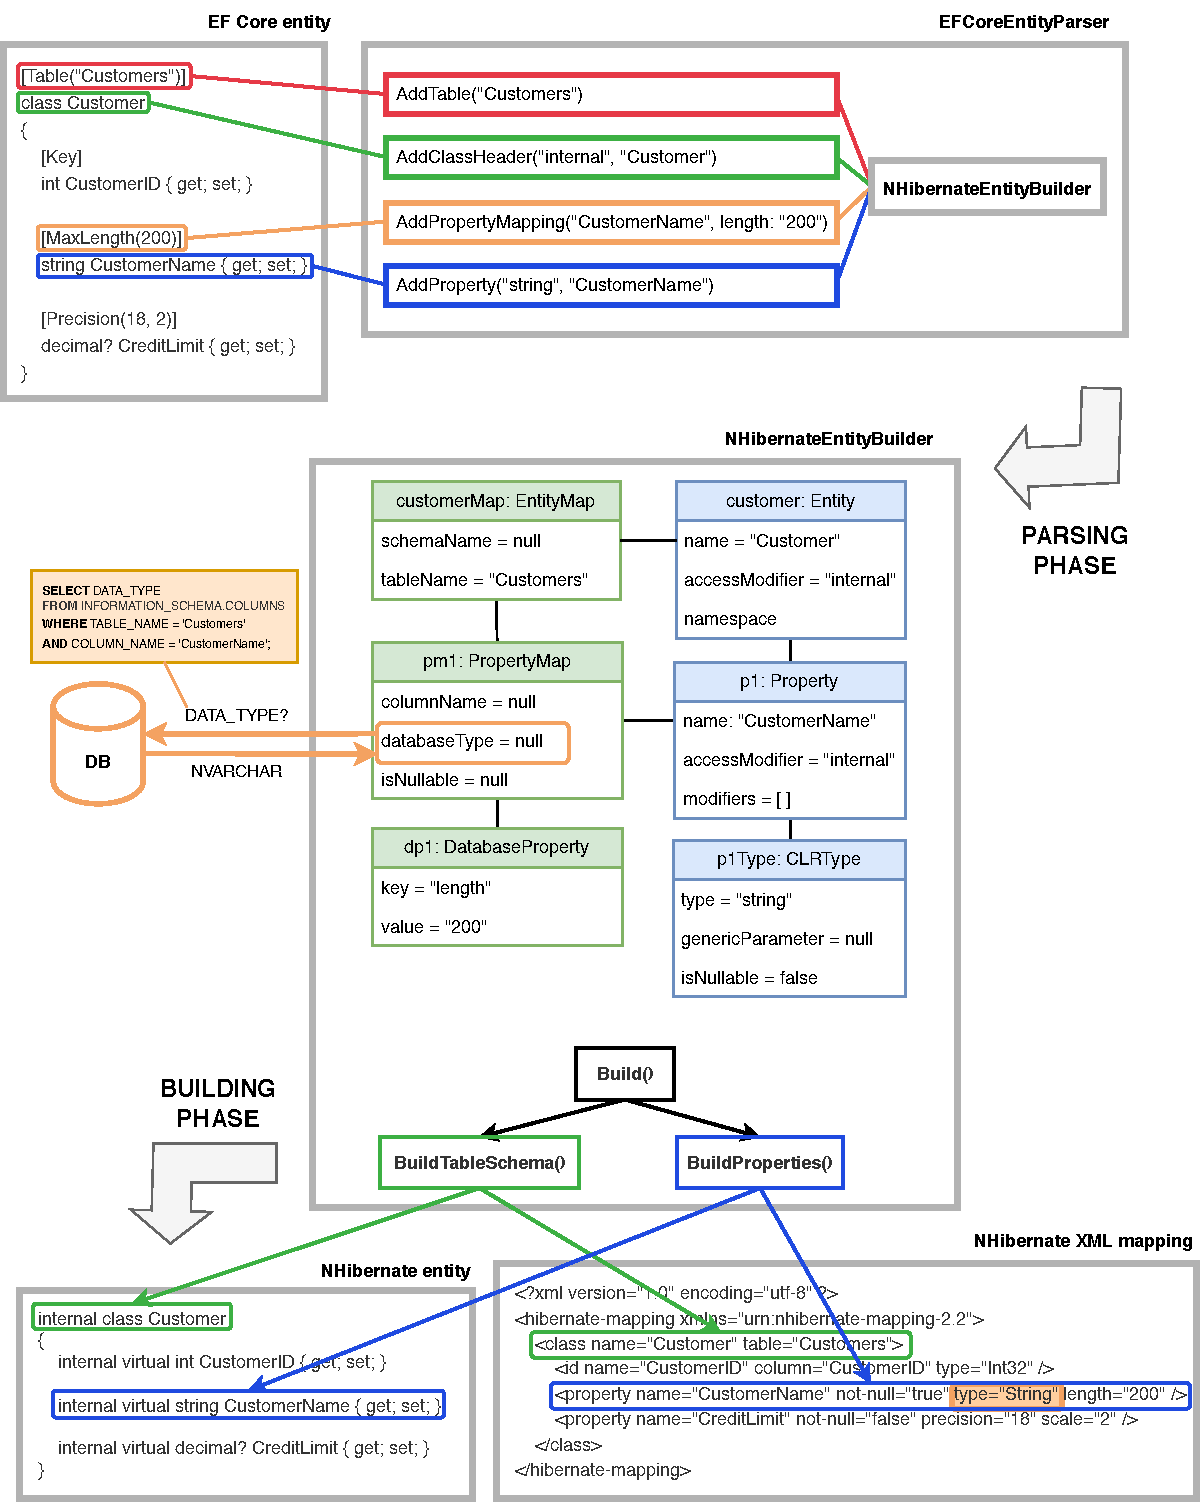
\includegraphics[width=\textwidth]{thesis/img/thesis/04_parsing_building.drawio.pdf}
  \caption{Translation of \acrshort{efcore} entity mapping to NHibernate.}
  \label{fig:abstract_ir}
\end{figure}
